% Documentation of template:
% https://mirror.koddos.net/CTAN/macros/latex/contrib/beamer-contrib/themes/metropolis/doc/metropolistheme.pdf

\documentclass{beamer}
\usetheme[progressbar=head, numbering=fraction, background=light, block=fill]{metropolis}% Use metropolis theme
\usepackage{preamble}

\title{On the Decomposition of Persistence Modules}
\date{\today}
\author{Yoav Eshel}
\institute{Supervisor: Dr. Magnus Botnan,\\Vrije Universiteit Amsterdam}


\begin{document}
    \maketitle
    \begin{frame}{Contents}
        \tableofcontents
    \end{frame}
    \section{Persistent Homology}
    \begin{frame}{One-parameter persistent homology}
        \begin{columns}[T]
            \begin{column}{0.5\textwidth}
                \begin{itemize}
                    \uncover<1-4>{\item Start with a point cloud data $X$.}
                    \uncover<2-4>{\item Draw an $\varepsilon$-ball around each point and denote the resulting topological space by $X_\varepsilon$.}
                    \uncover<3-4>{\item Compute the $i$-th homology group, $H_i(X_\varepsilon)$, with coefficients in a field $\mathbf{k}$.}
                    \uncover<4-4>{\\\alert{Idea}: if $H_i(X_\varepsilon)\neq 0$, then $X_\varepsilon$ has an $i$-dimensional hole.}
                \end{itemize}
            \end{column}
            \begin{column}{0.5\textwidth}
                \only<1>{\begin{figure}
                    \centering
                    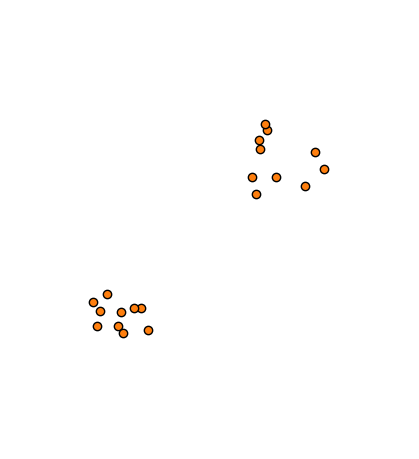
\includegraphics[scale=0.4]{figures/pointCloud_noBalls.png}
                \end{figure}}
                \uncover<2-4>{\begin{figure}
                    \centering
                    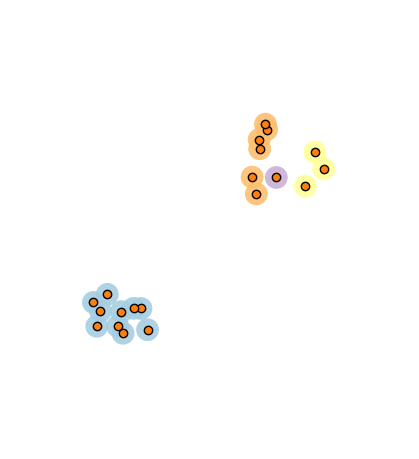
\includegraphics[scale=0.4]{figures/pointCloud_smallBalls.png}
                \end{figure}}
            \end{column}
        \end{columns}
    \end{frame}
    \begin{frame}{One-parameter persistent homology}
        For each $\varepsilon>0$ we have a vector space $H_i(X_\varepsilon)$.\pause

        For each $\delta<\varepsilon$ we have a linear map $\iota_{\delta,\varepsilon}\colon H_i(X_\delta)\to H_i(X_\varepsilon)$ induced by the inclusion $X_\delta\hookrightarrow X_\varepsilon$.\pause

        \begin{definition}
            The collection $\{H_i(X_\varepsilon),\iota_{\delta,\varepsilon}\}$ is called the \alert{$i$-dimensional persistent homology} of $X$.
        \end{definition}
    \end{frame}

    \begin{frame}{Persistence modules}
        \begin{definition}
            A \alert{persistence module} (over $\Rb$) is a functor $M:\Rb\to\Vect$, where we view the partially ordered set (poset) $\Rb$ as a category in the natural way ($a\leq b\iff a\to b$)
        \end{definition}\pause

        \begin{example}
            \[ \Rb:\cdots\to -1\to 0\to 1\to 0\to\cdots \]
            \[ M:\cdots\to\mathbf{k}\xrightarrow{[1,0]^T}\mathbf{k}^2\xrightarrow{[1,1]}\mathbf{k}\to\cdots \]
        \end{example}\pause

        We say that $M$ is \alert{pointwise finite dimensional (pfd)} if $\dim M(t)<\infty$ for all $t\in\Rb$
    \end{frame}
    
    \begin{frame}{Structure theorem}
        \begin{definition}
            Let $[a,b)\subset\Rb$. An \alert{interval module} $\Ib_{[a,b)}$ is the persistence module which has $\Ib_{[a,b]}(t)=\mathbf{k}$ for $t\in[a,b)$ (and 0 otherwise) and $\Ib_{[a,b)}(t\to s)=\id_{\mathbf{k}}$ for $a\leq t\leq s<b$ (and 0 otherwise).
        \end{definition}\pause
        \begin{theorem}
            Let $M$ be a pfd persistence module. Then there exists a unique colletion of intervals $\mathcal{B}=\{[a_i, b_i)\subset\Rb\mid i=1,\dots, n\}$ such that
            \[M\cong\bigoplus_{A\in\mathcal{B}}\Ib_{A}.\]
        \end{theorem}
        \cite{BotnanCrawley_2018}\pause
        
        We call $\mathcal{B}$ the \alert{barcode} of $M$.
    \end{frame}

    \begin{frame}{An example}
        \begin{figure}
            \centering
            \begin{tikzpicture}
                \foreach \Value in {1,2,3,4,5,6,7,8,9,10,11}
                  \node<\Value> (img\Value) {\includegraphics[width=0.9\linewidth]{./figures/barcode/barcode\Value}};
            \end{tikzpicture}
        \end{figure}              
    \end{frame}

    \begin{frame}{Limitations of one parameter persistent homology}
        \begin{figure}[h]
            \centering
            \begin{subfigure}{.45\textwidth}
              \centering
              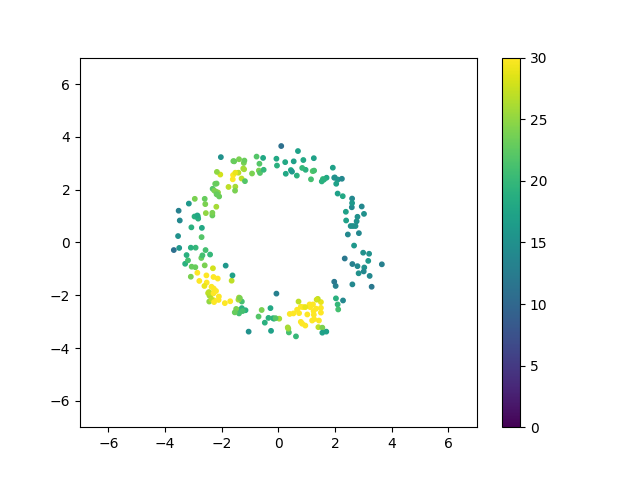
\includegraphics[width=.9\linewidth]{./figures/circle}
              \label{fig:circle}
            \end{subfigure}
            \begin{subfigure}{.45\textwidth}
              \centering
              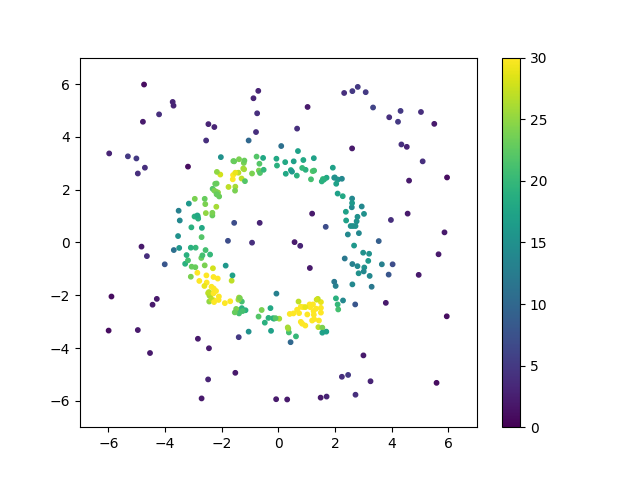
\includegraphics[width=.9\linewidth]{./figures/circle-all-points}
              \label{fig:circle-all-points}
            \end{subfigure}
            \begin{subfigure}{.45\textwidth}
              \centering
              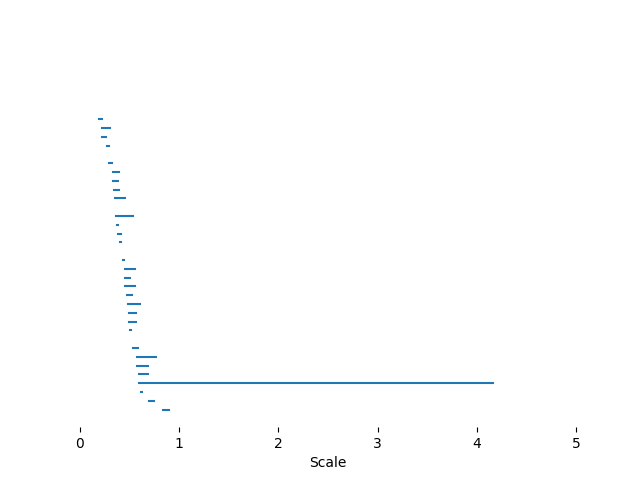
\includegraphics[width=.9\linewidth]{./figures/barcode-circle}
              \label{fig:barcode-circle}
            \end{subfigure}
            \begin{subfigure}{.45\textwidth}
              \centering
              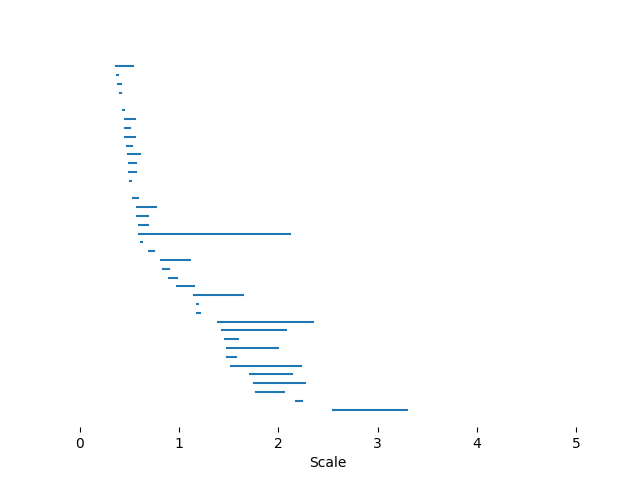
\includegraphics[width=.9\linewidth]{./figures/barcode-all-points}
              \label{fig:barcode-all}
            \end{subfigure}
            \caption{\cite{botnanLesnick_2022}}
            \label{fig:circles-full}
        \end{figure}
    \end{frame}


    \begin{frame}{Multiparameter persistence}
        Recall: a persistence module is a functor $M\colon \Rb\to\Vect$.\pause
        
        What if we replace $\Rb$ by $\Rb^2$? Or $\Nb^2$? Or $\Rb^n$? Do we still have a "barcode"?\pause
        
        \begin{figure}
            \centering
            \begin{subfigure}{.45\textwidth}
                \centering
                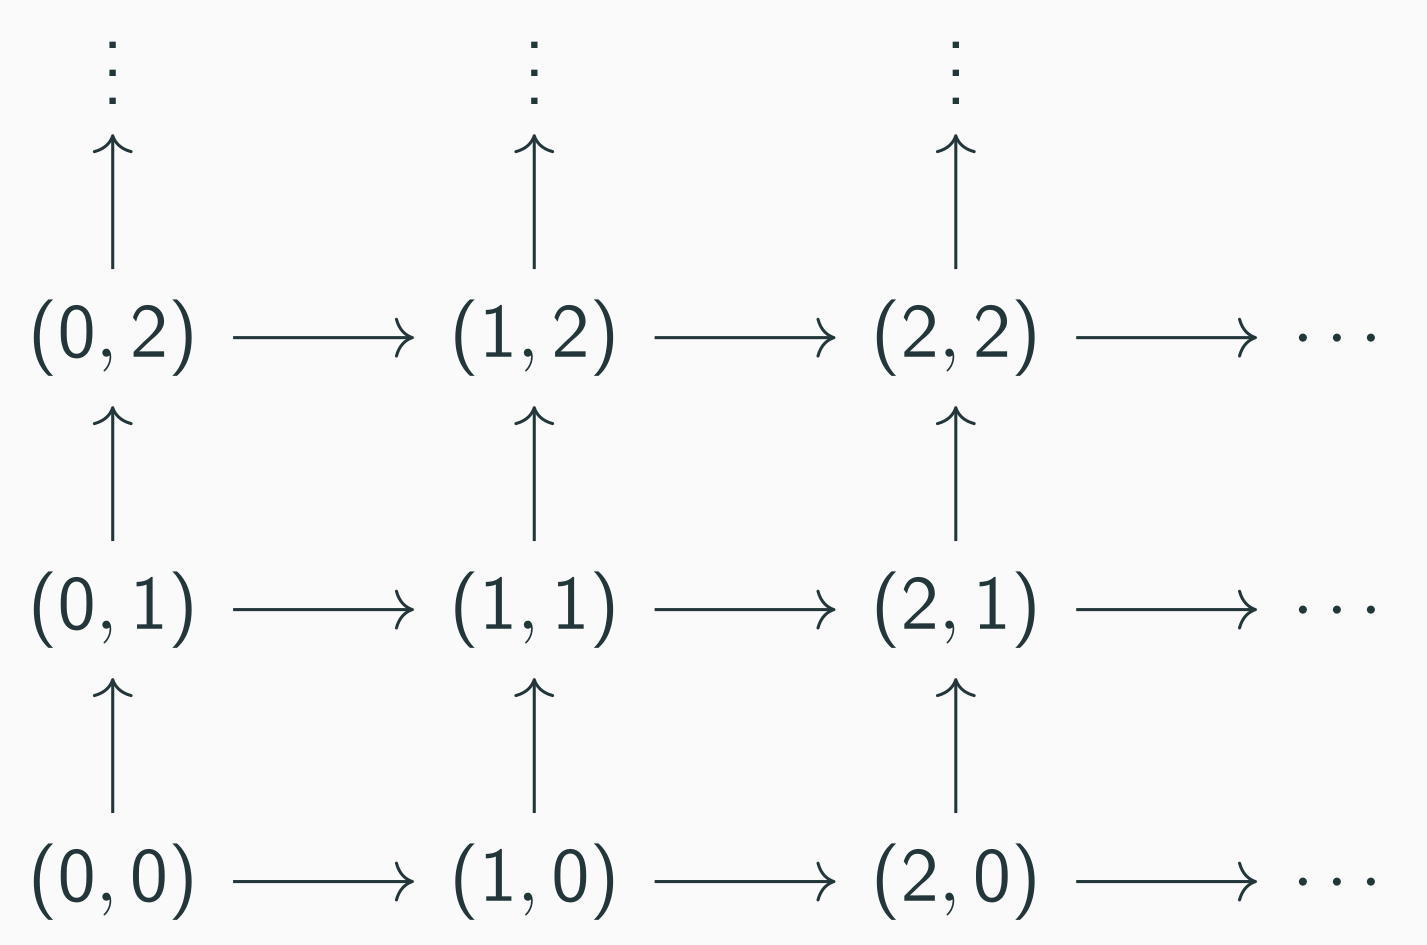
\includegraphics[width=.9\linewidth]{./figures/N2}
                \caption{The poset $\Nb^2$}
            \end{subfigure}
            \begin{subfigure}{.45\textwidth}
                \centering
                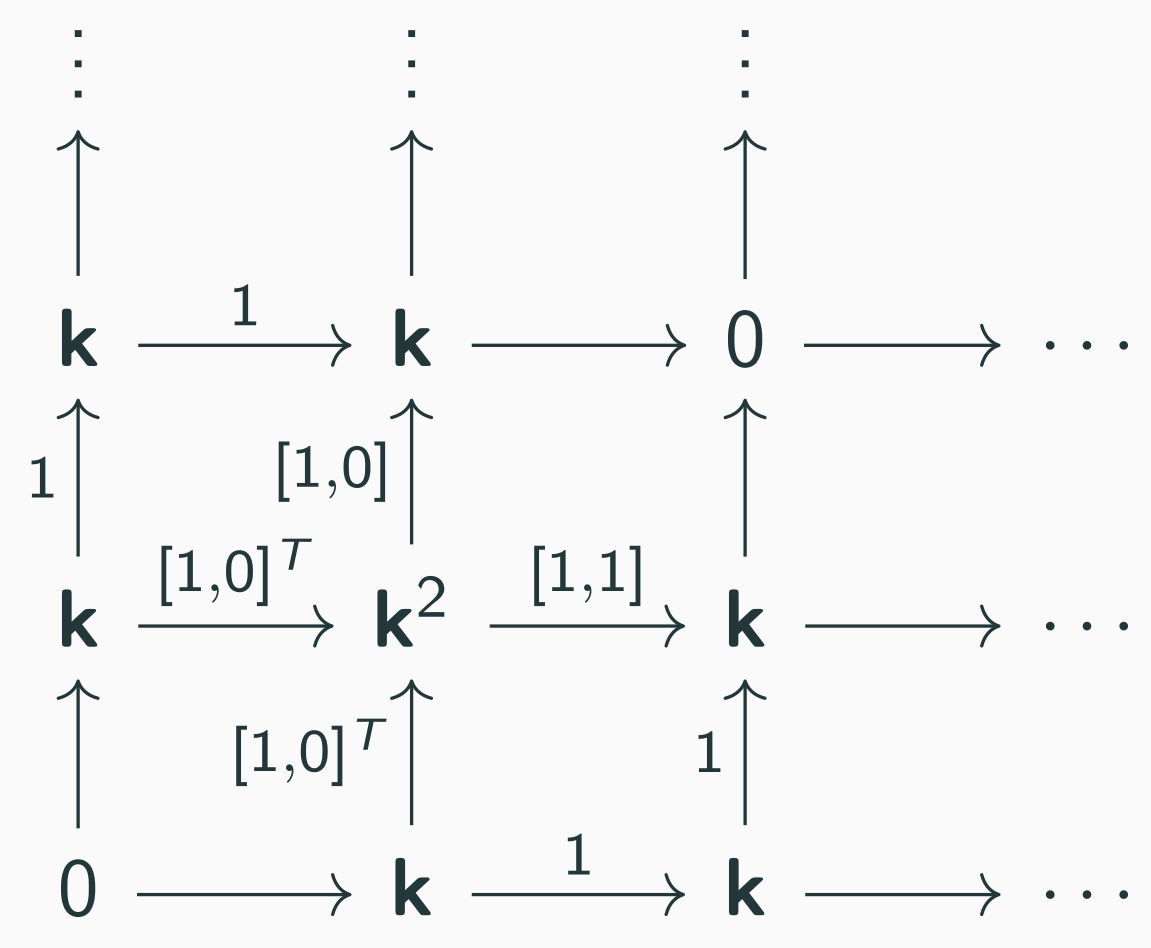
\includegraphics[width=.9\linewidth]{./figures/repN2}
                \caption{A persistence module over $\Nb^2$}
            \end{subfigure}
        \end{figure}
    \end{frame}
    
    \begin{frame}{Main theorem}
        Unfortunately, there is no similar complete discrete invariant for multidimensional persistence \cite{gunnar_2007}.\pause

        \begin{theorem}
            Let $P$ be a small category and $M\colon P\to\Vect$ a pfd persistence module. 
            Then $M$ has an essentially unique decomposition into indecomposable summands.
        \end{theorem}
    \end{frame}
    
    \section{Existence of Decomposition}
    \begin{frame}{Overview}
        \resizebox{!}{7cm}{%
            \begin{tikzpicture}[node distance=2cm]
                \node(tensor)[wide]{The Tensor Product};\pause
                \node(homtensor)[wide, below of =tensor, xshift=-3cm]{Tensor-Hom Adjunction};
                \draw [->] (tensor) -- (homtensor);\pause
                \node(puresubmodule)[process, below of =tensor, xshift=3cm]{Pure-Exact Sequences};
                \draw [->] (tensor) -- (puresubmodule);\pause
                \node(pureinjective)[process, below of =puresubmodule, xshift=-3cm]{Pure-Injective Module};
                \node(directpure)[process,below of =puresubmodule]{Direct Summand is a Pure Submodule};
                \node(chainpure)[process, below of =puresubmodule, xshift=3cm]{Union of Chain of Pure Submodules is Pure};
                \draw [->] (puresubmodule) -- (pureinjective);
                \draw [->] (puresubmodule) -- (directpure);
                \draw [->] (puresubmodule) -- (chainpure);\pause
                \node(modulepureinjective)[wide, below of =pureinjective, xshift=-2cm]{Every pfd Persistence Module is Pure Injective};
                \draw [->] (homtensor) -- (modulepureinjective);
                \draw [->] (pureinjective) -- (modulepureinjective);\pause
                \node(indecomposable)[wide, below of=modulepureinjective, xshift=3.5cm, yshift=-1cm]{Every pfd Persistence Module has an Indecomposable Summand};
                \draw [->] (modulepureinjective) -- (indecomposable);
                \draw [->] (chainpure) -- (indecomposable);
                \draw [->] (directpure) -- (indecomposable);\pause
                \node(sumindecomposable)[wide, right of =indecomposable, xshift=3cm]{Every pfd Persistence Module is a Direct Sum of indecomposable};
                \draw [->] (indecomposable) -- (sumindecomposable);
                % \node()[]{};
            \end{tikzpicture}}
            
            \only<8>{Based on idea by William Crawley-Boevey}
    \end{frame}

    \begin{frame}{The Tensor Product and Duality}
        Let $M\colon P\to\Vect, N\colon P^{\text{op}}\to\Vect$.\pause
        
        The tensor product $N\otimes_P M$ is defined by the universal property
        \begin{center}
            \begin{tikzcd}[ampersand replacement=\&]
                N\times M \arrow[r, "\varphi"] \arrow[rd, "\forall"'] \& N\otimes_P M \arrow[d, "!\exists", dotted] \\
                                                                      \& V                                        
            \end{tikzcd}
        \end{center}\pause
        Pointwise duality gives a contravariant, exact functor $D:\RepP\to\RepPop$
        \begin{center}
            \begin{tikzcd}[ampersand replacement=\&]
                M:  \& \mathbf{k} \arrow[r] \& \mathbf{k}^2 \arrow[r]     \& \mathbf{k}^3               \\
                DM: \& \mathbf{k}^*         \& (\mathbf{k}^2)^* \arrow[l] \& (\mathbf{k}^3)^* \arrow[l]
            \end{tikzcd}
        \end{center}
    \end{frame}

    \begin{frame}{Tensor-Hom Adjunction}
        And we have a tensor-hom adjunction
        \[ \Hom_{\mathbf{k}}(N\otimes_P M,\mathbf{k})\cong\Hom_P(M, DN) \]
    \end{frame}

    \begin{frame}{Pure submodules and pure-exact sequences}
        A short exact sequence $0\to A\to B\to C\to 0$ is \alert{pure-exact} if
        \[ 0\to M\otimes_P A\to M\otimes_P B\to M\otimes_P C\to 0 \]
        is exact for all $M$.\pause

        A submodule $M'\subseteq M$ is \alert{pure} in $M$ if the sequence
        \[ 0\to M'\to M\to M/M'\to 0 \]
        is pure-exact.
    \end{frame}
    
    \begin{frame}{Pure-injectivity}
        A module $M$ is \alert{pure-injective} if one of the equivalent conditions hold:\pause
        \begin{enumerate}
            \item $\Hom_P(-, M)$ preserves pure-exact sequences\pause
            \item Every pure exact sequence $0\to M\to M'\to M''\to 0$ splits.
        \end{enumerate}
    \end{frame}

    \begin{frame}{Pure-injectivity}
        \begin{lemma}
            Every pfd persistence module $M$ is pure injective
        \end{lemma}
    \end{frame}

    \begin{frame}{Every pfd persistence module has an indecomposable summand}
        Let $x\in M$. The set $S=\{N\subseteq M\mid N\text{ is pure in }M\text{ and }x\not\in N\}$ has a maximal element $N$.\pause
        
        The canonical exact sequence $0\to N\to M\to M/N\to 0$ is split, i.e. $M\cong N\oplus M/N$.\pause
        
        $M/N$ is non-zero since $x\in M/N$ and indecomposable by the maximality of $N$.
    \end{frame}


    \section{Uniqueness of Decomposition}
    \begin{frame}{Uniqueness}
         \begin{theorem}
            If $M=\bigoplus_{i\in I}M_i=\bigoplus_{j\in J}N_j$ are two direct sum decompositions of $M$ into indecomposables, then there exists an isomorphism $\varphi\colon I\to J$ such that $M_i\cong N_{\varphi(i)}$ for all $i\in I$.
        \end{theorem}\pause
        Proof relies on
        \begin{itemize}
            \item A pfd persistence module is indecomposable if and only if it has a local endomorphism ring\pause
            \item An adaptation of the Krull-Remak-Schmidt-Azumaya Theorem
        \end{itemize}
    \end{frame}

    




    % \begin{frame}{Existence of decomposition}
        
    % \end{frame}
    % \begin{frame}{Existence of decomposition}
    %     \begin{lemma}
    %         Every non-zero pfd persistence module is a direct sum of indecomposables.
    %     \end{lemma}\pause
    %     \begin{proof}
    %         \begin{itemize}
    %             \item The set $S=\{N\subseteq M\mid N\text{ is indecomposable}\}$ is non-empty by the previous Lemma.\pause
    %             \item The set $U=\{I\subseteq S\mid \bigoplus_{N\in I}N\text{ is a direct summand of } M\}$ has a maximal element $I$.\pause
    %             \item By the maximality of $I$, $M=\bigoplus_{N\in I}N$.
    %         \end{itemize}
    %     \end{proof}
    % \end{frame}

   
    % \begin{frame}{Uniqueness of decomposition}
    %     Important facts\pause
    %     \begin{itemize}
    %         \item A pfd persistence module is indecomposable if and only if it has a local endomorphism ring.\pause
    %         \item If $M=\bigoplus_{i\in I}M_i$ with $M_i$ indecomposable and $\eta\colon M\to M$ idempotent and nonzero, then there exists $i\in I$ such that $\eta(M_i)\cong M_i$ and $\eta(M_i)$ is a direct summand of $M$.\pause
    %         \item Any indecomposable direct summand of $M$ is isomorphic to $M_i$ for some $i\in I$.
    %     \end{itemize}
    % \end{frame}

    % \begin{frame}{Uniqueness of decomposition}
    %     \begin{theorem}
    %         If $M=\bigoplus_{i\in I}M_i=\bigoplus_{j\in J}N_j$ are two direct sum decompositions of $M$ into indecomposables, then there exists an isomorphism $\varphi\colon I\to J$ such that $M_i\cong N_{\varphi(i)}$ for all $i\in I$.
    %     \end{theorem}
    %     \begin{proof}
    %         \begin{itemize}
    %             \item Introduce equivalence relation on $I$: $i_1\sim i_2$ if and only if $M_{i_1}\cong M_{i_2}$. Similarly, for $J$.\pause
    %             \item By considering the composition $M\xrightarrow{\pi_i} M_i\xrightarrow{\iota_i}M$ we conclude that each $M_i$ is isomorphic to $N_j$ for some $j\in J$ and conversely.\pause
    %             \item Hence, we can identify $K=I/\sim$ with $J/\sim$. Let $I_k\subseteq I$ (resp. $J_k\subseteq J$) denote the equivalence class of $k\in K$.\pause
    %             \item Left to prove that $\abs{I_k}=\abs{J_k}$ for all $k\in K$.
    %         \end{itemize}
    %     \end{proof}
    % \end{frame}
    
    \section{Conclusion}
    \begin{frame}[standout]
        Thank you for your attention
    \end{frame}
    

    \bibliographystyle{apalike}
    \bibliography{references}
\end{document}